\chapter{Learning and Memory}
\label{ch:learning}

\textit{Learning is the problem of changing weights from experience. This chapter asks how Hebbian updates store associations, how interference limits memory, and why sparsity can improve capacity in binary-synapse systems.}

% ============================================================
\section{Plasticity and Learning Rules}
\label{sec:plasticity}
% ============================================================

The weights in a neural network are not fixed---they change with experience. This is \emph{synaptic plasticity}\index{synaptic plasticity}, and it is the physical basis of learning and memory. The question for modelers is: what rule governs how weights change?

Three broad paradigms exist. In \emph{supervised learning}\index{supervised learning}, a teacher provides the correct output for each input, and the weights are adjusted to reduce the error. In \emph{unsupervised learning}\index{unsupervised learning}, no teacher is available; the network discovers statistical structure in the inputs on its own. In \emph{reinforcement learning}\index{reinforcement learning}, the network receives a scalar reward signal and must figure out which actions led to reward. All three paradigms appear in neuroscience, but the oldest and most influential idea is Hebbian learning, which is unsupervised.

% ============================================================
\section{Hebbian Learning}
\label{sec:hebbian}
% ============================================================

In 1949, Donald Hebb proposed a remarkably simple principle: if neuron $A$ repeatedly helps fire neuron $B$, the synapse from $A$ to $B$ should get stronger. The modern shorthand is ``cells that fire together, wire together.'' Mathematically, the simplest Hebbian rule\index{Hebbian learning} is
%
\begin{equation}
  \Delta w_i = \eta\, x_i\, y
  \label{eq:hebb}
\end{equation}
%
where $x_i$ is the presynaptic activity, $y$ is the postsynaptic activity, and $\eta$ is a small learning rate. The weight increases when pre- and postsynaptic neurons are coactive and does not change when either is silent.

This rule is \emph{local}\index{local learning rule}: each synapse only needs information available at its own location---the activities of the neurons it connects. No global error signal is required. This is biologically attractive, because a synapse in the brain cannot easily access information from distant parts of the network.

\subsection{Learning an association}

Hebbian learning can link two previously unrelated stimuli. Suppose a visual neuron already responds to the sight of food (its weights from visual inputs are already strong). Now we present the sight and smell together. The visual stimulus drives the neuron to fire, and because the odor inputs are coactive with the output, their weights increase. After training, the odor alone can drive the neuron. The network has learned an association.

This is the computational analogue of classical conditioning: pairing a conditioned stimulus with an unconditioned one transfers the response. The Hebbian rule provides a synaptic mechanism.

% ============================================================
\section{The Perceptron as Associative Memory}
\label{sec:perceptron-memory}
% ============================================================

We now ask a precise quantitative question: how many input--output associations can a single perceptron store using Hebbian learning?

Suppose we have $N_s$ patterns to store. Each pattern is a pair $(\vec{u}^{(m)}, v^{(m)})$, where $\vec{u}^{(m)} \in \{-1, +1\}^{N_u}$ is a random binary input vector and $v^{(m)} \in \{-1, +1\}$ is the desired output. The Hebbian weight vector is the sum of outer products:

\begin{keyequation}[Hebbian Weight Vector]
\begin{equation}
  \vec{w} = \frac{1}{N_u}\sum_{m=1}^{N_s} v^{(m)}\,\vec{u}^{(m)}
  \label{eq:hebb-weight}
\end{equation}
\tcblower
$\vec{u}^{(m)}$: input pattern $m$, \quad
$v^{(m)}$: desired output, \quad
$N_u$: input dimension, \quad
$N_s$: number of stored patterns.
\end{keyequation}

\noindent Each stored association contributes a term $v^{(m)}\vec{u}^{(m)}$ to the weight vector. The normalization by $N_u$ keeps the weights from growing with input dimension.

\subsection{Signal and noise}

What happens when we present a stored input $\vec{u}^{(n)}$? The activation is
%
\begin{equation}
  \vec{w} \cdot \vec{u}^{(n)} = v^{(n)} + \eta^{(n)}
  \label{eq:signal-noise}
\end{equation}
%
where the first term is the correct output (the ``signal'') and the second term is crosstalk from all the other stored patterns:
%
\begin{equation}
  \eta^{(n)} = \frac{1}{N_u}\sum_{m \neq n} v^{(m)}\bigl(\vec{u}^{(m)} \cdot \vec{u}^{(n)}\bigr)
  \label{eq:crosstalk}
\end{equation}

\begin{derivation}[Signal--noise decomposition]
Expand $\vec{w} \cdot \vec{u}^{(n)}$ using \cref{eq:hebb-weight}:
\begin{align*}
  \vec{w} \cdot \vec{u}^{(n)}
    &= \frac{1}{N_u}\sum_{m=1}^{N_s} v^{(m)}\bigl(\vec{u}^{(m)} \cdot \vec{u}^{(n)}\bigr) \\[4pt]
    &= \frac{1}{N_u}\,v^{(n)}\underbrace{\bigl(\vec{u}^{(n)} \cdot \vec{u}^{(n)}\bigr)}_{= N_u}
      \;+\; \frac{1}{N_u}\sum_{m \neq n} v^{(m)}\bigl(\vec{u}^{(m)} \cdot \vec{u}^{(n)}\bigr) \\[4pt]
    &= v^{(n)} + \eta^{(n)}
\end{align*}
The signal term is exactly $v^{(n)}$ because $\vec{u}^{(n)} \cdot \vec{u}^{(n)} = N_u$ (each component is $\pm 1$). The noise term $\eta^{(n)}$ is a sum of $N_s - 1$ random dot products.
\end{derivation}

\noindent The classification is correct when $\operatorname{sign}(\vec{w} \cdot \vec{u}^{(n)}) = v^{(n)}$, which requires $|{\eta^{(n)}}| < 1$. The question is: how likely is this to hold?

\subsection{Noise statistics and capacity}

Each dot product $\vec{u}^{(m)} \cdot \vec{u}^{(n)}$ is a sum of $N_u$ independent random $\pm 1$ terms. When patterns are random and uncorrelated, the central limit theorem\index{central limit theorem} tells us that $\eta^{(n)}$ is approximately Gaussian with mean zero and variance
%
\begin{equation}
  \sigma_\eta^2 = \frac{N_s - 1}{N_u}
  \label{eq:noise-variance}
\end{equation}

\noindent The noise grows with the number of stored patterns and shrinks with the input dimension. Retrieval is reliable when $\sigma_\eta \ll 1$, which requires $N_s \ll N_u$. A common rule of thumb is that performance remains good up to roughly $N_s \approx 0.2\,N_u$.

This is the \emph{capacity}\index{capacity!Hebbian perceptron} of the Hebbian perceptron. It is far from optimal---the Hebbian rule wastes capacity because it treats all patterns equally and does not try to minimize interference. With a more sophisticated learning algorithm (for instance, the perceptron learning rule with error correction), the capacity can be pushed up to $N_s \approx N_u$ for large $N_u$. But the Hebbian rule has the virtue of being local, one-shot, and biologically plausible.

% ============================================================
\section{Sparse Coding and Binary Synapses}
\label{sec:sparse}
% ============================================================

We now consider a different regime: a network with binary synapses ($w_{ij} \in \{0, 1\}$) and sparse activity patterns. This model, closely related to the Willshaw network\index{Willshaw network}, can store far more patterns per synapse than the dense Hebbian scheme.

\subsection{Setup}

The network has $N$ neurons in both input and output populations, with random connectivity: each pair of neurons has a synapse with probability $\rho$. Each pattern activates $M$ out of $N$ neurons, with $M \ll N$ (sparse coding\index{sparse coding}). The learning rule is simple: set $w_{ij} = 1$ if both neuron $i$ (input) and neuron $j$ (output) are active during the presentation of a pattern. A synapse, once turned on, is never turned off.

Each association imprints at most $M^2$ synapses. The total number of synapses available is $\rho N^2$. A crude upper bound on the number of storable patterns is therefore
%
\begin{equation}
  P \leq \rho\Bigl(\frac{N}{M}\Bigr)^{\!2}
  \label{eq:sparse-capacity}
\end{equation}

\subsection{The error criterion}

The real constraint comes from false positives: a neuron that should be silent but fires because too many of its synapses have been turned on by other patterns. The probability that a particular potential synapse has been set to $1$ by at least one of the $P$ stored patterns grows with $P$. For an output neuron that should be off, we need all $M$ of its incoming active synapses to happen to be zero---otherwise it could falsely activate.

The expected number of erroneously active output neurons scales as $N p_{\text{on}}^M$, where $p_{\text{on}}$ denotes the probability that a given potential synapse has been switched on. Requiring fewer than one error on average gives the criterion
%
\begin{equation}
  N p_{\text{on}}^M < 1
  \label{eq:error-criterion}
\end{equation}
%
Taking logarithms and solving for $M$:
%
\begin{equation}
  M > \frac{-\ln N}{\ln p_{\text{on}}}
  \label{eq:min-sparsity}
\end{equation}

\noindent Since $\ln p_{\text{on}} < 0$ (because $p_{\text{on}} < 1$), the right-hand side is positive. Sparser patterns (smaller $M$) increase the capacity in \cref{eq:sparse-capacity}, but $M$ cannot be too small or \cref{eq:error-criterion} is violated. The optimal sparsity balances these two forces.

\subsection{The sparsity--capacity tradeoff}

Substituting the optimal $M$ back into the capacity formula gives a maximum storage that scales as
%
\begin{equation}
  P_{\max} \propto \frac{\rho(\ln p_{\text{on}})^2\, N^2}{(\ln N)^2}
  \label{eq:max-capacity}
\end{equation}
%
This is a remarkable result. The capacity grows as $N^2$ (up to logarithmic corrections), far faster than the $O(N)$ scaling of the dense Hebbian perceptron. The price is that each pattern carries very little information (only $M \ll N$ active bits), so the total information stored per synapse is more modest. But the number of distinct \emph{patterns} is enormous.

The tradeoff is fundamental: if $M$ is too small, each pattern is so sparse that it barely uses the network's resources, but the error rate is low. If $M$ is too large, patterns overlap heavily and retrieval fails. The optimum sits between these extremes.

\begin{figure}[h]
\centering
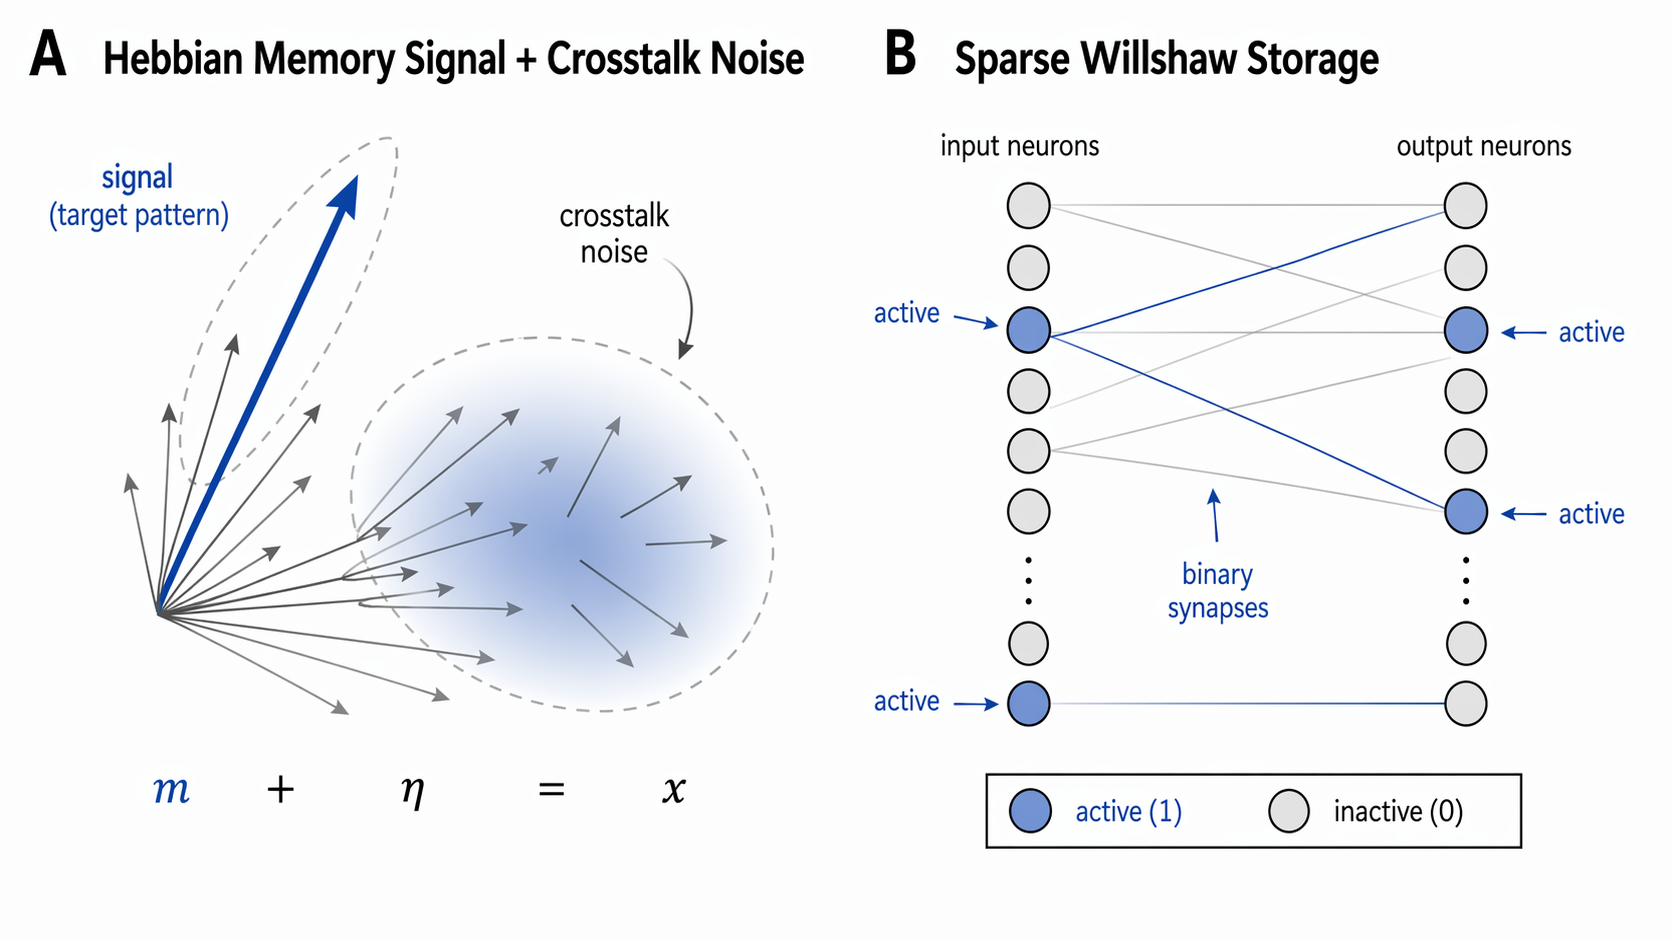
\includegraphics[width=\textwidth]{figures/mns-learning-memory.png}
\caption{Two capacity mechanisms. Dense Hebbian recall separates the desired signal from random crosstalk noise, while sparse Willshaw-style storage uses low activity and binary coactivation to reduce false positives.}
\label{fig:learning-memory}
\end{figure}


\begin{chaptersummary}

\begin{center}
\renewcommand{\arraystretch}{1.6}
\begin{tabularx}{\textwidth}{@{}l X X@{}}
  \toprule
  \textbf{Concept} & \textbf{Equation} & \textbf{Key Insight} \\
  \midrule
  Hebbian rule &
  $\Delta w_i = \eta\, x_i\, y$ &
  Local, correlation-based weight update \\
  %
  Hebbian weight vector &
  $\displaystyle \vec{w} = \frac{1}{N_u}\sum_m v^{(m)}\vec{u}^{(m)}$ &
  Sum of input--output outer products \\
  %
  Retrieval &
  $\vec{w} \cdot \vec{u}^{(n)} = v^{(n)} + \eta^{(n)}$ &
  Signal plus crosstalk noise \\
  %
  Noise variance &
  $\displaystyle \sigma_\eta^2 = \frac{N_s - 1}{N_u}$ &
  More patterns $\Rightarrow$ more interference \\
  %
  Sparse capacity &
  $\displaystyle P \leq \rho\Bigl(\frac{N}{M}\Bigr)^{\!2}$ &
  Sparse codes store more patterns \\
  %
  Error criterion &
  $N p_{\text{on}}^M < 1$ &
  Constrains minimum sparsity \\
  \bottomrule
\end{tabularx}
\end{center}

\end{chaptersummary}

\begin{conceptquestions}
  \item Distinguish between supervised, unsupervised, and reinforcement learning. Which category does the Hebbian rule fall into, and why?

  \item The Hebbian rule $\Delta w_i = \eta\, x_i\, y$ is called a ``local'' learning rule. What does locality mean here, and why is it biologically important?

  \item Naive Hebbian learning can cause weights to grow without bound. Why? What mechanisms could prevent this in a biological network?

  \item Explain how Hebbian learning can produce an association between two previously unrelated stimuli (e.g., the sight and smell of food). Walk through the learning process step by step.

  \item In the retrieval equation $\vec{w} \cdot \vec{u}^{(n)} = v^{(n)} + \eta^{(n)}$, where does the noise term $\eta^{(n)}$ come from? Decompose it and explain why its variance grows with the number of stored patterns.

  \item The noise variance is $\sigma_\eta^2 = (N_s - 1)/N_u$. What does this formula tell you about the tradeoff between the number of stored patterns $N_s$ and the input dimension $N_u$? Roughly how many patterns can be stored reliably?

  \item Why is the central limit theorem needed to analyze the crosstalk noise? What conditions must hold for it to apply, and what does it tell us about the distribution of $\eta^{(n)}$?

  \item The Hebbian rule is ``not optimal'' for storage capacity. What does this mean, and what property of the Hebbian rule causes it to waste capacity compared to an optimal algorithm?

  \item In the sparse binary synapse model, why does making patterns sparser increase the number of storable patterns? What prevents us from making patterns arbitrarily sparse?

  \item The sparse model uses binary synapses that can only be turned on, never off. What problem does this create as the number of stored patterns grows, and how does the error criterion $Np_{\text{on}}^M < 1$ address it?

  \item The dense Hebbian perceptron stores $O(N)$ patterns, while the sparse binary model stores $O(N^2/\log^2 N)$ patterns. Where does this dramatic improvement come from? Is the total \emph{information} stored per synapse also dramatically better, or is there a tradeoff?
\end{conceptquestions}
